\documentclass[11pt]{article}
\usepackage[a4paper,margin=1cm]{geometry}
\usepackage{helvet}
\renewcommand{\familydefault}{\sfdefault}
\usepackage[T1]{fontenc}
\usepackage[utf8]{inputenc}
\usepackage{array}
\usepackage{xcolor}
\usepackage[hidelinks]{hyperref}
\usepackage{enumitem}
\usepackage{pifont}
\usepackage{amssymb}
\usepackage{graphicx}
\usepackage[absolute,overlay]{textpos}
\usepackage{titlesec}
\usepackage{tcolorbox} % ✅ For rounded colored boxes
\usepackage{fontawesome}
\usepackage{contour}
\contourlength{0.6pt} % thickness of the outline


\setlength{\parindent}{0pt}

% ==== Rounded colored section titles ====
\newcommand{\SectionBox}[1]{%
\vspace{6pt}
\begin{tcolorbox}[
    colback=black!10,    % background color
    colframe=black!10,   % border same as background
    boxrule=0pt,        % no visible border
    arc=8pt,            % rounded corners
    left=5pt, right=5pt, top=4pt, bottom=4pt,
    width=\textwidth,   % full width
    halign=center,      % ✅ centers text horizontally
    valign=center       % ✅ centers vertically in case of multiple lines
]
\textbf{\large #1}
\end{tcolorbox}
\vspace{-1pt}
}

% ==== Section commands ====
\newcommand{\ProfileSection}[0]{\SectionBox{PROFILE}}
\newcommand{\EducationSection}[0]{\SectionBox{EDUCATION}}
\newcommand{\ExperienceSection}[0]{\SectionBox{PROFESSIONAL EXPERIENCE}}
\newcommand{\ProjectsSection}[0]{\SectionBox{PROJECTS}}
\newcommand{\CertificationsSection}[0]{\SectionBox{CERTIFICATIONS}}
\newcommand{\SkillsSection}[0]{\SectionBox{SKILLS}} % <-- NEW COMMAND
\newcommand{\LanguagesSection}[0]{\SectionBox{LANGUAGES}}

\begin{document}
\pagestyle{empty} 

% ==== Photo ====
\begin{textblock*}{3cm}(16.7cm,0.84cm)
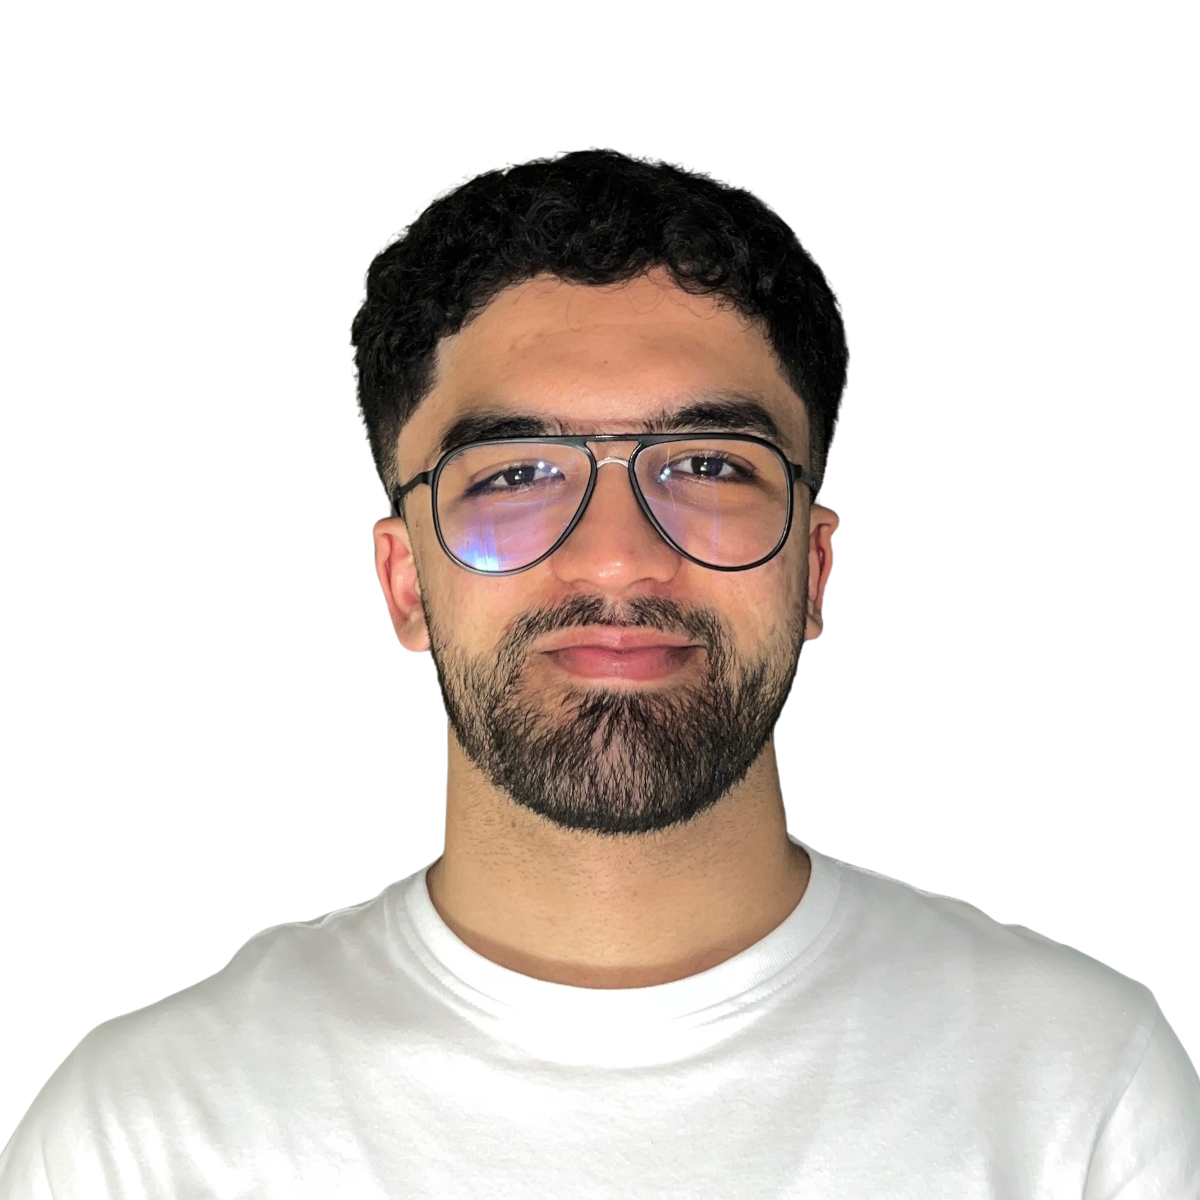
\includegraphics[width=3.3cm]{Profil-removebg.png}
\end{textblock*}

% ==== Header inside a rounded box ====
\begin{tcolorbox}[
    colback=black!10,       % background color
    colframe=black!10,      % border color
    arc=10pt,              % rounded corners (all sides)
    boxrule=0pt,           % no visible border
    width=\textwidth,      % full page width
    left=10pt, right=10pt, top=8pt, bottom=6pt
]
{\Huge\bfseries AZIZ BELHADJ SAYAR}\\[8pt]
\contour{white}{{\fontsize{18pt}{18pt}\selectfont\textcolor{blue}{Computer Science Student}}}\\[-5pt]

\renewcommand{\arraystretch}{0.9}
\setlength{\tabcolsep}{6pt}
{\fontsize{9}{10}\selectfont
\begin{tabular*}{0.6\textwidth}{@{\extracolsep{\fill}} l l l}
    \textcolor{blue}{\faPhone} \textbf{+33 6 52 64 32 02} &
    \textcolor{blue}{\faLinkedin} \href{https://linkedin.com/in/azizbelhadjsayar}{\textbf{linkedin.com/in/azizbelhadjsayar}} &
    \textcolor{blue}{\faEnvelope} \href{mailto:aziz.belhadjsayar@etud.univ-evry.fr}{\textbf{aziz.belhadjsayar@etud.univ-evry.fr}} \\
    \textcolor{blue}{\faMapMarker}  \textbf{Paris, France} &
    \textcolor{blue}{\faGithub} \href{https://github.com/azizbelhadjsayar}{\textbf{github.com/azizbelhadjsayar}} \\
\end{tabular*}
}
\end{tcolorbox}

\vspace{-0.2cm}

% ==== Profile ====
\ProfileSection
Motivated and detail-oriented student passionate about Business Intelligence and software development.  
Currently pursuing a Master’s degree in \textbf{Software Engineering for the Web} at \textbf{Université Paris-Saclay}.

% ==== Education ====
\EducationSection
\noindent
\begin{tabular*}{\textwidth}{@{\extracolsep{\fill}} l r}
\textbf{Université Paris-Saclay} & \textbf{Paris, France \faMapMarker} \\
\textbf{MSc 1 – Software Engineering for the Web} & \textbf{2024 -- 2025 \faCalendar} \\
\end{tabular*}
\begin{itemize}[leftmargin=*,itemsep=1pt,topsep=1pt,parsep=0pt,label=\textcolor{blue}{\faArrowCircleRight}]
    \item Courses: Software Engineering, Web Development, Databases
\end{itemize}

\vspace{0.2cm}

\noindent
\begin{tabular*}{\textwidth}{@{\extracolsep{\fill}} l r}
\textbf{IHEC Carthage} & \textbf{Tunis, Tunisia \faMapMarker} \\
\textbf{Bachelor’s in Business Computing (Business Intelligence)} & \textbf{2021 -- 2024 \faCalendar} \\
\end{tabular*}
\begin{itemize}[leftmargin=*,itemsep=1pt,topsep=1pt,parsep=0pt,label=\textcolor{blue}{\faArrowCircleRight}]
    \item Courses: Business Intelligence, SQL, Data Analysis
\end{itemize}

% ==== Experience ====
\ExperienceSection
\noindent
\begin{tabular*}{\textwidth}{@{\extracolsep{\fill}} l r}
\textbf{Tech Solutions} & \textbf{Paris, France \faMapMarker} \\
\textbf{Junior Web Developer} & \textbf{2023 -- 2024 \faCalendar} \\
\end{tabular*}
\begin{itemize}[leftmargin=*,itemsep=1pt,topsep=1pt,parsep=0pt,label=\textcolor{blue}{\faArrowCircleRight}]
    \item Developed an internal web application using Python and Angular
    \item Optimized SQL database performance
\end{itemize}

% ==== Projects ====
\ProjectsSection
\noindent
\begin{tabular*}{\textwidth}{@{\extracolsep{\fill}} l r}
\textbf{Interactive Dashboard (Python, Streamlit)} \href{https://github.com/azizbelhadjsayar/dashboard-data}{\textcolor{blue}{\faGithub}} & \textbf{2024 \faCalendar} \\
\end{tabular*}
\begin{itemize}[leftmargin=*,itemsep=1pt,topsep=1pt,parsep=0pt,label=\textcolor{blue}{\faArrowCircleRight}]
    \item Data analysis and visualization of real-world datasets with interactive charts.
\end{itemize}

\vspace{0.2cm}
\noindent
\begin{tabular*}{\textwidth}{@{\extracolsep{\fill}} l r}
\textbf{Gesture-Controlled Game (Python, OpenCV, MediaPipe)} \href{https://github.com/azizbelhadjsayar/dashboard-data}{\textcolor{blue}{\faGithub}} & \textbf{2023 \faCalendar} \\
\end{tabular*}
\begin{itemize}[leftmargin=*,itemsep=1pt,topsep=1pt,parsep=0pt,label=\textcolor{blue}{\faArrowCircleRight}]
    \item Interactive game using real-time hand movement detection.
\end{itemize}

\vspace{0.2cm}
\noindent
\begin{tabular*}{\textwidth}{@{\extracolsep{\fill}} l r}
\textbf{Library Management App (Java Swing, MySQL)} \href{https://github.com/azizbelhadjsayar/dashboard-data}{\textcolor{blue}{\faGithub}} & \textbf{2023 \faCalendar} \\
\end{tabular*}
\begin{itemize}[leftmargin=*,itemsep=1pt,topsep=1pt,parsep=0pt,label=\textcolor{blue}{\faArrowCircleRight}]
    \item Desktop app featuring barcode generation, scanning, and email alerts.
\end{itemize}

\vspace{0.2cm}
\noindent
\begin{tabular*}{\textwidth}{@{\extracolsep{\fill}} l r}
\textbf{HR Management App (C\#, .NET, SQL Server)} \href{https://github.com/azizbelhadjsayar/dashboard-data}{\textcolor{blue}{\faGithub}} & \textbf{2022 \faCalendar} \\
\end{tabular*}
\begin{itemize}[leftmargin=*,itemsep=1pt,topsep=1pt,parsep=0pt,label=\textcolor{blue}{\faArrowCircleRight}]
    \item Full CRUD management of employees, locations, departments, and jobs.
\end{itemize}

% ==== Certifications ====
% ==== Certifications ====
\CertificationsSection
\href{https://www.coursera.org/professional-certificates/google-data-analytics}{Google Data Analytics Professional Certificate} 
\textcolor{blue}{\Large •} 
\href{https://www.datacamp.com/courses/data-visualization-with-python}{Data Visualization with Python – DataCamp} 
\textcolor{blue}{\Large •} 
\href{https://www.hackerrank.com/skills-verification/sql_intermediate}{SQL (Intermediate) – HackerRank} 
\textcolor{blue}{\Large •} 
\href{https://www.kaggle.com/learn/intro-to-machine-learning}{Introduction to Machine Learning – Kaggle} 
\textcolor{blue}{\Large •} 
\href{https://www.coursera.org/learn/machine-learning}{Machine Learning – Stanford University} 
\textcolor{blue}{\Large •} 
\href{https://www.coursera.org/learn/neural-networks-deep-learning}{Neural Networks and Deep Learning – DeepLearning.AI} 
\textcolor{blue}{\Large •} 
\href{https://www.coursera.org/specializations/python}{Python for Everybody – University of Michigan} 
\textcolor{blue}{\Large •} 
\href{https://www.freecodecamp.org/learn/javascript-algorithms-and-data-structures/}{JavaScript Algorithms and Data Structures – freeCodeCamp} 
\textcolor{blue}{\Large •} 
\href{https://www.udemy.com/course/angular-complete-guide/}{Angular Complete Guide – Udemy}


% ==== Skills ====
% ==== Skills (The fix is here) ====
\SkillsSection
\vspace{0.2cm} % Reduce space after the header box to keep it tight
\noindent\parbox[t]{\textwidth}{ % <-- Encapsulate entire block for flow isolation
    \tcbset{
        on line,
        colback=gray!20,
        colframe=gray!60,
        arc=4pt,
        % Tighter padding and height for a sleek look
        top=1pt, bottom=1pt, 
        left=4pt, right=4pt,
        height=16pt,
        valign=center,
        baseline,
        % Allows width to adjust to content while setting a minimum for small words
        width=auto,
        box align=center
    }

    \noindent\parbox{\textwidth}{ % Ensures the list starts flush left and handles wrapping correctly
        \tcbox{Python}\hskip 3pt%
        \tcbox{Java}\hskip 3pt%
        \tcbox{C\#}\hskip 3pt%
        \tcbox{SQL}\hskip 3pt%
        \tcbox{JavaScript}\hskip 3pt%
        \tcbox{Angular}\hskip 3pt%
        \tcbox{Flask}\hskip 3pt%
        \tcbox{Streamlit}\hskip 3pt%
        \tcbox{OpenCV}\hskip 3pt%
        \tcbox{MediaPipe}\hskip 3pt%
        \tcbox{Git/GitHub}\hskip 3pt%
        \tcbox{Docker}\hskip 3pt%
        \tcbox{SQLite}\hskip 3pt%
        \tcbox{MySQL}\hskip 3pt%
        \tcbox{Excel}\hskip 3pt%
        \tcbox{Power BI}\hskip 3pt%
        \tcbox{Problem Solving}\hskip 3pt%
        \tcbox{Teamwork}\hskip 3pt%
        \tcbox{Communication}\hskip 3pt%
        \tcbox{Time Management}%
    }
} % <-- End of the encapsulation block


% ==== Languages ====
\LanguagesSection
% ==== Languages Content (Forced to single line without warning) ====
\hbadness=10000 % <-- Temporarily ignores horizontal spacing warnings
\textbf{English:} C2 – \href{https://cert.efset.org/6YsT6y}{\underline{EF SET C2} \faLink} \textbf{ | }
\textbf{French:} C2 – \href{https://drive.google.com/file/d/1yojzT_8XB7gIulaIKh8TSYeOl8NBXxpR/view}{\underline{TCF C2} \faLink} \textbf{ | }
\textbf{Arabic:} Native

\end{document}
